\documentclass{beamer}
\usepackage{amsmath}
\usepackage{amssymb}
\usepackage{amsthm}                                        
\usepackage{textcomp}     
\usepackage{xcolor}
\usepackage{listings} 
\usetheme{Madrid}
\title{Facial Keypoint Detection with Quaternion Convolutional Neural Networks}
\author{ZHANG HUAKANG\and LI JIALIN \and YU HANG}
\date{\today}
\begin{document}

\begin{frame}
    \titlepage
\end{frame}
\begin{frame}
    \frametitle{Table of Content}
    \tableofcontents
\end{frame}
\section{Introduction}
\begin{frame}{Introduction}
Facial Key Points (FKPs) detection is an important and challenging problem in the field of computer vision, which involves detecting FKPs like centers and corners of eyes, nose tip, etc.
% The problem is to predict the (x, y) real-valued co-ordinates in the space of image pixels of the FKPs for a given face image.
FKPs detection can be applied in tracking faces in images and videos, analysis of facial expressions, detection of dysmorphic facial signs for medical diagnosis, face recognition, etc.

In the past few years, advancements in FKPs detection are made by the application of deep convolutional neural network (DCNN), which is a special type of feed-forward neural network with shared weights and local connectivity. Not only in FKPs detection, but in other computer vision tasks, CNN is widely used and becomes more and more mature in recent years.
\end{frame}

\begin{frame}{Introduction}
CNN still has some drawbacks, like when dealing with the color images,general CNNs just treat the RGB three channels as three unrelated feature maps. For each kernel it just sums up the outputs corresponding to different channels and ignores the complicated interrelationship between them.  We may lose important structural information of color and obtain non-optimal representation of color image.

Focusing on the problems mentioned above, we are going to propose a model using on FKPs called quaternion convolutional neural network which represents a color in  the quaternion domain. Its conventional kernel, pooling layer and full connected layer will be replace with the operation of quaternion algebra. 

% We are also going to built a cascade QCNN model 
\end{frame}


\section{Related Works}
\subsection{Facial Keypoint Detection}
\begin{frame}{Related Works}{Facial Keypoint Detection}
Facial keypoints detection is a problem of estimating the position of eyes, nose, and mouth in a facial image. This problem, also known as face alignment, has been widely studied for many years in the field of computer vision because of its relevance to various face analysis applications such as face recognition , face attribute recognition, head pose estimation, and 3D face modeling systems.

In order to develop a detector that is robust to disturbances and environmental changes, existing studies have proposed a feature extraction algorithm\cite{1717463,5539992} or a method that can directly model the shape of the face\cite{Cootes2000AnIT,10.1007/BFb0054760}. Various CNN-based regression methods have been proposed like deep convolutional network cascade for facial point detection\cite{6619290}.
\end{frame}
\subsection{CNN}
\begin{frame}{Related Works}{CNN}
Convolutional neural network is one of the most successful models in many vision tasks. Since the success of LeNet\cite{726791} in digit recognition, great progresses have been made. AlexNet\cite{NIPS2012_c399862d} is the first deep CNN that greatly outperforms all past models in image classification task. Then, a number of models with deep and complicated structures are proposed, such as VGG\cite{brusilovsky:simonyan2014very} and ResNet\cite{7780459}.A traditional convolutional neural network consists of one or several convolutional layers, followed by some fully-connected layers of neurons. Each convolution block usually produces feature maps by four steps, \emph{e.g.}, convolution, batch normalization, non-linear activation, and pooling.
\end{frame}

\subsection{Quaternion}
\begin{frame}{Related Works}{Quaternion}
Quaternion is a kind of number system extending the complex numbers which was first described by William Rowan Hamilton in 1843. A quaternion $\hat{q}$ in the quaternion domain $\mathbb{H}$, \emph{i.e}, $q\in \mathbb{H}$, can be represented as $\hat{q}=q_0+q_1i+q_2j+q_3k$, where $q_n\in \mathbb{R}$ for $n=0,1,2,3$, and the imaginary units $i,j,k$ obey the quaternion rules that $i^2=j^2=k^2=ijk=-1$. 
\end{frame}
\begin{frame}{Related Works}{Quaternion}
Similar to real numbers, we can define a series of operations for quaternions:
\begin{itemize}
    \item Addition:
    \begin{equation*}
        \begin{split}
            \hat{p}+\hat{q}=&(p_0+q_0)+(p_1+q_1)i
                            +(p_2+q_2)j+(p_3+q_3)k
        \end{split}
    \end{equation*}
    \item Scalar multiplication: $$\lambda \hat{q}=\lambda q_0+\lambda q_1i+\lambda q_2j+\lambda q_3k$$
    \item Element multiplication: 
    \begin{equation*}
        \begin{split}
            \hat{p}\hat{q}=&(p_0q_0-p_1q_1-p_2q_2-p_3q_3)
                        +(p_0q_1+p_1q_0+p_2q_3-p_3q_2)i\\
                        +&(p_0q_2-p_1q_3-p_2q_0-p_3q_1)j
                        +(p_0q_3+p_1q_2-p_2q_1-p_3q_0)k
        \end{split}
    \end{equation*}
    \item Conjugation: $$\hat{q}^*=q_0-q_1i-q_2j-q_3k$$
\end{itemize}
\end{frame}
\begin{frame}{Related Works}{Quaternion}
These quaternion operations can be used to represent rotations in a three-dimensional space. Suppose that we want to rotate a 3D vector $\textbf{q}=[q_1,q_2,q_3]^T$ to get new vector $\textbf{p}=[p_1,p_2,p_3]^T$, with an angle $\theta$ and along a rotation axis $\textbf{w}=[w_1,w_2,w_3]^T, w_1^2+w_2^2+w_3^2=1$. Such a rotation is equivalent to the following quaternion operation: 
\begin{equation}
    \hat{p}=\hat{w}\hat{q}\hat{w}^*
\end{equation}
where $\hat{q}= 0 + q_1i + q_2j + q_3k$, $\hat{p}= 0 + p_1i + p_2j + p_3k$ and 
\begin{equation}
    \hat{w}=\cos\frac{\theta}{2}+\sin\frac{\theta}{2}(w_1i + w_2j + w_3k)
\end{equation}
\end{frame}
\begin{frame}{Related Works}{Quaternion}
Since its convenience in representing rotations of three-dimensional vectors, in the field of computer vision and image processing, quaternion-based methods show its potentials in many tasks. For example, quaternion principal component analysis network\cite{ZENG2016416} and quaternion-based sparse representation of color image\cite{6607436} have been proven to be better in extracting more representative features for color images.
\end{frame}





\section{Motivation}
\begin{frame}{Motivation}
In recent years, real-valued CNN has been widely used in the field of computer vision. CNN has a good performance in all kinds of tasks, the image classification and retrieval, target location detection, object segmentation and face recognition. In face recognition, each person's facial features vary greatly, and for the same person, due to the size, position, posture and so on, the change will be different. This is more difficult under different conditions, such as lighting, viewing angle, occlusion, etc\cite{9065279}. Convolutional neural network with deep structure can solve these problems well.
\end{frame}
\begin{frame}{Motivation}
But CNN also has some drawbacks. Its natural judgment of color images is defective\cite{parcollet:hal-02107644}.
In the specific case of image recognition, a good model has to efficiently encode local relations within the input features,such as between the Red, Green, and Blue channels of a single pixel.


In particular, traditional real value CNN treats pixels as three separate values. In other words, in the training process of CNN, both internal implicit relation and global implicit relation are considered at the same level.

Therefore, CNN may lose some information that depends on the internal relationship of the image.
\end{frame}
\begin{frame}{Motivation}
To solve this problem, we propose to replace CNN with QCNN, which treats a pixel as a multidimensional entity.
In particular, each color pixel in a color image is represented as a quaternion, and accordingly, the image is represented as a quaternion matrix rather than three independent real-valued matrices.
QCNN enhances the ability of the model to learn the internal relations of pixels and external relations.
% And It significantly reduces the number of neural parameters.
% In the experimental comparison between CNN and QCNN, the number of neural parameters in QCNN was reduced by 4 times\cite{parcollet:hal-02107644}.
\end{frame}
\section{Proposed method}
\subsection{Basic Architecture}
\begin{frame}{Proposed method}{Basic Architecture}
    \begin{figure}[H]
        \centering
        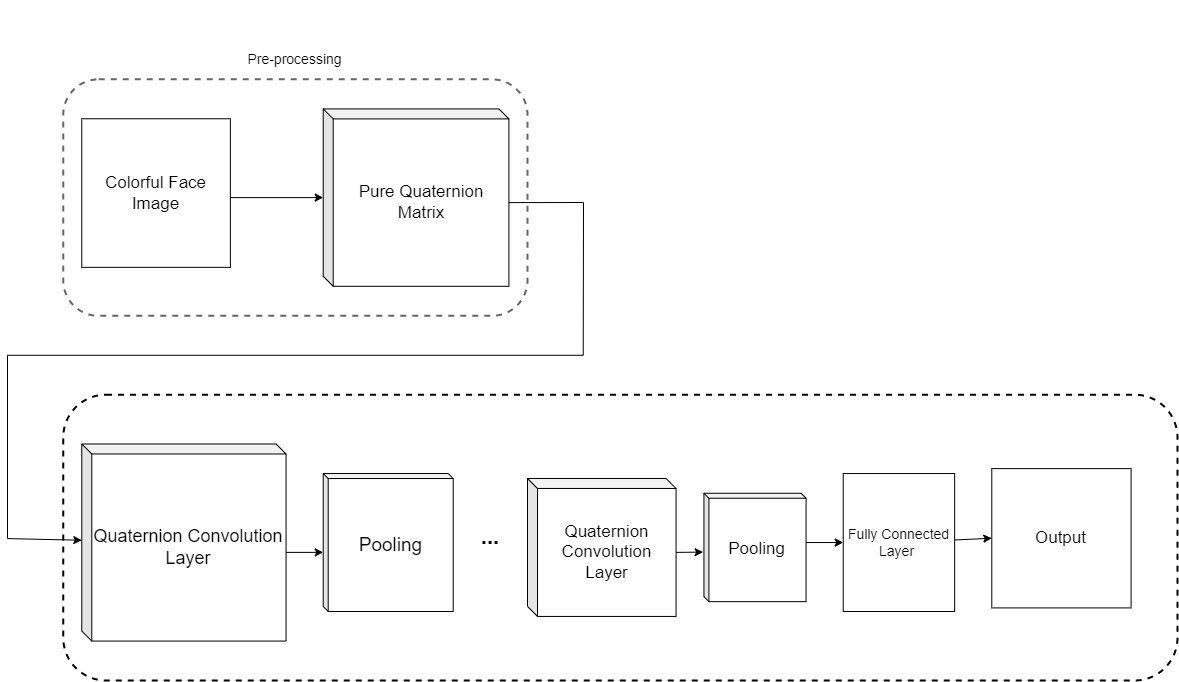
\includegraphics[width=\textwidth]{img/1.png}
        \caption{Architecture}
    \end{figure}
\end{frame}
\begin{frame}{Proposed method}{Pure Quaternion Matrix}
    Focusing on color image representation, our quaternion CNN treats a color image as a 2D pure quaternion matrix, denoted as $\hat{A}=[\hat{a}_{nn'}]\in \mathbb{H}^{N\times N}$ where $N$ represents the size of the image. In particular, the quaternion matrix $\hat{A}$ is 
    \begin{equation}
        \hat{A}=\mathbf{0}+\textbf{R}i+\textbf{G}j+\textbf{B}k,
    \end{equation}
    where $\textbf{R},\textbf{G},\textbf{B}\in \mathbb{R}^{N\times N}$ represent red, green and blue channels, respectively.
    \begin{figure}[H]
        \centering
        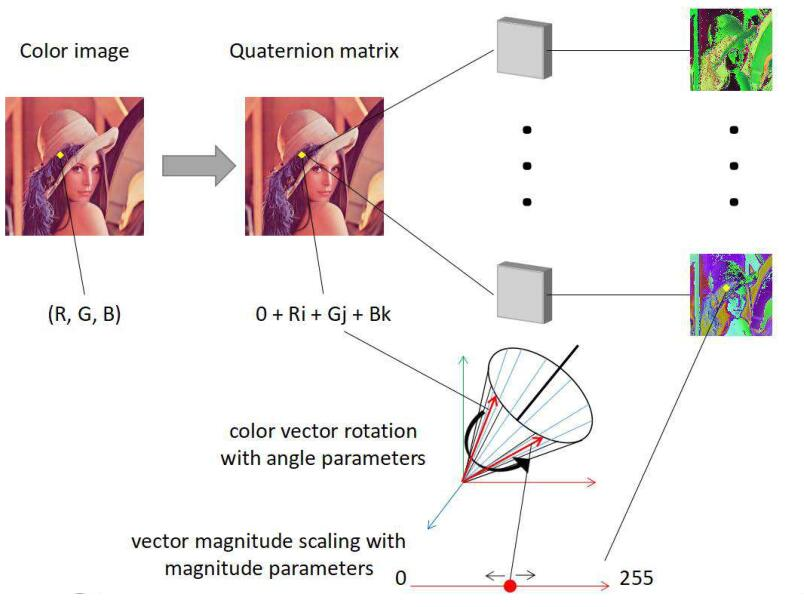
\includegraphics[width=0.4\textwidth]{img/2.jpg}
        \caption{Architecture}
    \end{figure}
\end{frame}
\subsection{Quaternion Convolution, Pooling \& Fully Connected Layer}
\begin{frame}{Proposed method}{Quaternion Convolution, Pooling \& Fully Connected Layer}
    \begin{itemize}
        \item \textbf{Quaternion Convolution Layer}: We are going to come up with a new quaternion convolution kernel and an operation between the input and kernel based on the quaternion rotation.\begin{itemize}
            \item Which axis the rotation should follow.
            \item How to determine the angle of rotation.
        \end{itemize}
        \item \textbf{Pooling Layer \& Fully Connected Layer }: We are going to come up with a new pooling layer and fully connected layer based on the quaternion algebra, \emph{e.g.}, addition, scalar multiplication and conjugation.
            \begin{itemize}
                \item Which pooling function in the real number domain can be extended to quaternion.
                \item How does the pooling operation work.
                \item How to define the fully connected layer.
            \end{itemize}
    \end{itemize}
\end{frame}
\subsection{Learning Quaternion CNNs}
\begin{frame}{Proposed method}{Learning Quaternion CNNs}
    \begin{itemize}
        \item \textbf{Backpropagation} is the key of training a network, which applies the chain rule to compute gradients of the parameters and updates them.
        \begin{itemize}
            \item How to define the loss function.
            \item How to get the backpropagation algorithm in QCNN?
        \end{itemize}
    \end{itemize}
\end{frame}

\subsection{Implement}
\begin{frame}{Proposed method}{Implement}
Similar to real-valued CNN, QCNN can be accelerated using parallel computing, which means training on GPU with thousands of cores will be faster than training on CPU with dozens of cores. Thus, we are going to develop our QCNN framework based on \emph{CUDA API} or a machine learning framework that supports GPU computing, \emph{e.g.} \emph{PyTorch}, \emph{Tensorflow}.
\end{frame}
\begin{frame}
    $$Thanks$$
\end{frame}
\begin{frame}
    $$Q\&A$$
\end{frame}
\bibliographystyle{ieeetr}
\bibliography{ref} 
\end{document}